% Appendix B: Detailed Diagrams

\chapter{Detailed Diagrams}

\section{System Architecture Diagrams}

\subsection{Complete System Architecture}

\begin{figure}[H]
\centering
\begin{tikzpicture}[node distance=2cm, auto]
  % Define styles
  \tikzstyle{component}=[rectangle, draw=black, fill=blue!10, text width=3cm, text centered, minimum height=1cm]
  \tikzstyle{external}=[rectangle, draw=black, fill=green!10, text width=3cm, text centered, minimum height=1cm]
  \tikzstyle{database}=[cylinder, draw=black, fill=red!10, text width=3cm, text centered, minimum height=1cm, shape border rotate=90]
  \tikzstyle{arrow}=[->, thick]

  % Mobile Layer
  \node[component] (mobile) {Flutter Mobile App};

  % Web Layer
  \node[component, below of=mobile] (web) {Angular Web App};

  % API Gateway
  \node[component, below of=web] (gateway) {JHipster API Gateway};

  % Microservices
  \node[component, left of=gateway, xshift=-3cm] (auth) {Auth Service};
  \node[component, below of=auth] (user) {User Service};
  \node[component, right of=gateway, xshift=3cm] (report) {Report Service};
  \node[component, below of=report] (template) {Template Service};

  % Database
  \node[database, below of=user, yshift=-1cm] (db) {PostgreSQL Database};

  % External Services
  \node[external, right of=report, xshift=2cm] (firebase) {Firebase Cloud Messaging};

  % Connections
  \draw[arrow] (mobile) -- (gateway);
  \draw[arrow] (web) -- (gateway);
  \draw[arrow] (gateway) -- (auth);
  \draw[arrow] (gateway) -- (report);
  \draw[arrow] (auth) -- (db);
  \draw[arrow] (user) -- (db);
  \draw[arrow] (report) -- (db);
  \draw[arrow] (template) -- (db);
  \draw[arrow] (report) -- (firebase);
\end{tikzpicture}
\caption{Complete RM System Architecture}
\label{fig:system_architecture}
\end{figure}

\subsection{Database Schema Diagram}

\begin{figure}[H]
\centering
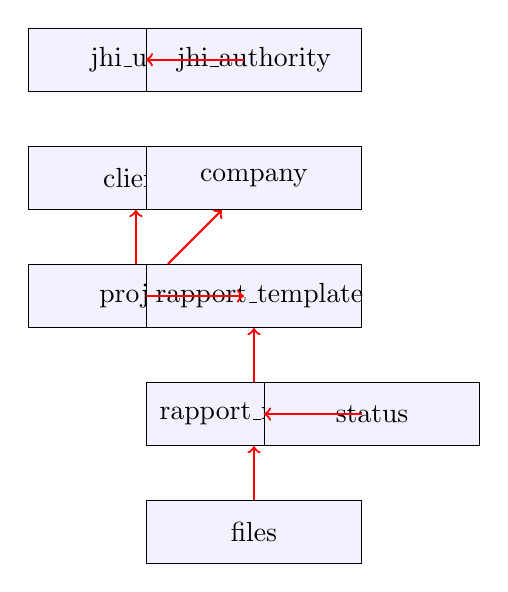
\begin{tikzpicture}[node distance=1.5cm, auto]
  % Define styles
  \tikzstyle{table}=[rectangle, draw=black, fill=blue!5, text width=2.5cm, text centered, minimum height=0.8cm]
  \tikzstyle{fk}=[->, thick, color=red]

  % Tables
  \node[table] (user) {jhi\_user};
  \node[table, right of=user] (authority) {jhi\_authority};
  \node[table, below of=user] (client) {client};
  \node[table, right of=client] (company) {company};
  \node[table, below of=client] (project) {projet};
  \node[table, right of=project] (template) {rapport\_template};
  \node[table, below of=template] (request) {rapport\_request};
  \node[table, right of=request] (status) {status};
  \node[table, below of=request] (files) {files};

  % Relationships
  \draw[fk] (user) -- (authority);
  \draw[fk] (project) -- (client);
  \draw[fk] (project) -- (company);
  \draw[fk] (template) -- (project);
  \draw[fk] (request) -- (template);
  \draw[fk] (request) -- (status);
  \draw[fk] (files) -- (request);
\end{tikzpicture}
\caption{Database Entity-Relationship Diagram}
\label{fig:database_schema}
\end{figure}

\section{Use Case Diagrams}

\subsection{Complete System Use Case Diagram}

\begin{figure}[H]
\centering
\begin{tikzpicture}[node distance=2cm, auto]
  % Define styles
  \tikzstyle{actor}=[rectangle, draw=black, fill=yellow!20, text width=2cm, text centered, minimum height=1cm]
  \tikzstyle{usecase}=[ellipse, draw=black, fill=green!10, text width=2.5cm, text centered, minimum height=0.8cm]
  \tikzstyle{arrow}=[->, thick]

  % Actors
  \node[actor] (technician) {Field Technician};
  \node[actor, below of=technician] (supervisor) {Project Supervisor};
  \node[actor, below of=supervisor] (coordinator) {Project Coordinator};
  \node[actor, below of=coordinator] (admin) {System Administrator};

  % Use Cases
  \node[usecase, right of=technician, xshift=3cm] (login) {User Authentication};
  \node[usecase, below of=login] (view) {View Interventions};
  \node[usecase, below of=view] (fill) {Fill Dynamic Forms};
  \node[usecase, below of=fill] (submit) {Submit Interventions};
  \node[usecase, right of=coordinator, xshift=3cm] (create) {Create Templates};
  \node[usecase, below of=create] (manage) {Manage Interventions};
  \node[usecase, below of=manage] (reports) {Generate Reports};

  % Relationships
  \draw[arrow] (technician) -- (login);
  \draw[arrow] (technician) -- (view);
  \draw[arrow] (technician) -- (fill);
  \draw[arrow] (technician) -- (submit);
  \draw[arrow] (coordinator) -- (create);
  \draw[arrow] (coordinator) -- (manage);
  \draw[arrow] (supervisor) -- (reports);
  \draw[arrow] (admin) -- (login);
\end{tikzpicture}
\caption{Complete System Use Case Diagram}
\label{fig:use_case_diagram}
\end{figure}

\section{Sequence Diagrams}

\subsection{Authentication Flow Sequence Diagram}

\begin{figure}[H]
\centering
\begin{lstlisting}
\newthread{user}{User}
\newthread{client}{Client App}
\newthread{gateway}{API Gateway}
\newthread{auth}{Auth Service}
\newthread{db}{Database}

\begin{call}{user}{client}{Enter credentials}
\end{call}

\begin{call}{client}{gateway}{POST /api/authenticate}
\end{call}

\begin{call}{gateway}{auth}{validateCredentials()}
\end{call}

\begin{call}{auth}{db}{findByLogin()}
\end{call}

\begin{callself}{db}{auth}{Return user}
\end{callself}

\begin{callself}{auth}{auth}{generateToken()}
\end{callself}

\begin{callself}{auth}{gateway}{Return token}
\end{callself}

\begin{callself}{gateway}{client}{200 OK + token}
\end{callself}

\begin{callself}{client}{client}{Store token}
\end{callself}
\end{lstlisting}
\caption{Authentication Flow Sequence Diagram}
\label{fig:auth_sequence}
\end{figure}

\section{State Diagrams}

\subsection{Intervention Lifecycle State Diagram}

\begin{figure}[H]
\centering
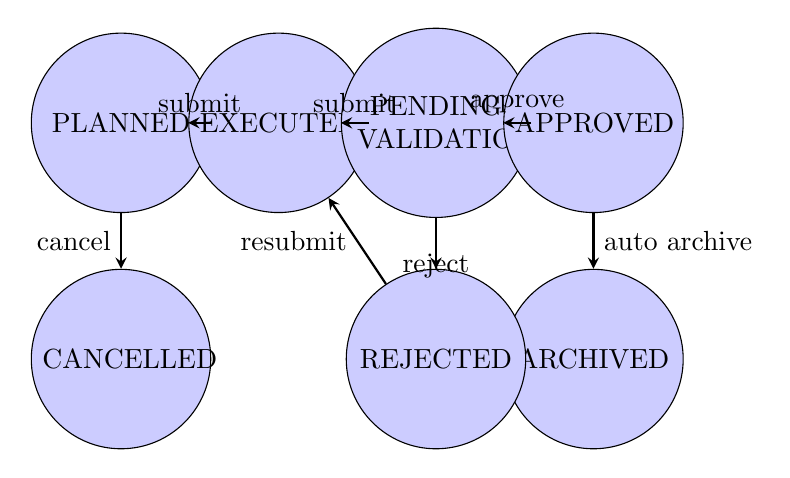
\begin{tikzpicture}[node distance=2cm, auto, >=stealth]
  % Define styles
  \tikzstyle{state}=[circle, draw=black, fill=blue!20, text width=2cm, text centered, minimum height=1cm]
  \tikzstyle{transition}=[->, thick]

  % States
  \node[state] (planned) {PLANNED};
  \node[state, right of=planned] (executed) {EXECUTED};
  \node[state, right of=executed] (validation) {PENDING\\VALIDATION};
  \node[state, right of=validation] (approved) {APPROVED};
  \node[state, below of=approved, yshift=-1cm] (archived) {ARCHIVED};
  \node[state, below of=planned, yshift=-1cm] (cancelled) {CANCELLED};
  \node[state, below of=validation, yshift=-1cm] (rejected) {REJECTED};

  % Transitions
  \draw[transition] (planned) -- node[above] {submit} (executed);
  \draw[transition] (planned) -- node[left] {cancel} (cancelled);
  \draw[transition] (executed) -- node[above] {submit} (validation);
  \draw[transition] (validation) -- node[above] {approve} (approved);
  \draw[transition] (validation) -- node[below] {reject} (rejected);
  \draw[transition] (approved) -- node[right] {auto archive} (archived);
  \draw[transition] (rejected) -- node[left] {resubmit} (executed);
\end{tikzpicture}
\caption{Intervention Lifecycle State Diagram}
\label{fig:intervention_states}
\end{figure}